% This LaTeX document needs to be compiled with XeLaTeX.
\documentclass[10pt]{article}
\usepackage[utf8]{inputenc}
\usepackage{multirow}
\usepackage{amsmath}
\usepackage{amsfonts}
\usepackage{amssymb}
\usepackage[version=4]{mhchem}
\usepackage{stmaryrd}
\usepackage{graphicx}
\usepackage[export]{adjustbox}
\graphicspath{ {./images/} }
\usepackage[fallback]{xeCJK}
\usepackage{polyglossia}
\usepackage{fontspec}
\usepackage{newunicodechar}
\setCJKmainfont{Noto Serif CJK TC}

\setmainlanguage{polish}
\setmainfont{CMU Serif}

\title{WYPELNIA ZDAJĄCY }

\author{}
\date{}


\newunicodechar{ı}{\ifmmode\imath\else{$\imath$}\fi}

\begin{document}
\maketitle
\begin{center}
\begin{tabular}{|l|l|}
\hline
Klasa & Nazwisko i imię \\
\hline
 &  \\
\hline
\end{tabular}
\end{center}

\section*{PRÓBNY EGZAMIN MATURALNY Z MATEMATYKI POZIOM PODSTAWOWY}
\begin{center}
\begin{tabular}{|c|c|}
\hline
\multirow[b]{5}{*}{\begin{tabular}{l}
Marzec 2022 \\
Czas pracy: 170 minut \\
Liczba punktów do uzyskania: 45 \\
\end{tabular}} & WYPELNIA ZESPÓt NADZORUJACCY \\
\hline
 & Uprawnienia zdajacego do: \\
\hline
 & dostosowania zasad oceniania \\
\hline
 & dostosowania w zw. z dyskalkulia \\
\hline
 & nieprzenoszenie zaznaczeñ na kartẹ \\
\hline
\end{tabular}
\end{center}

\section*{Instrukcja dla zdajqcego}
\begin{enumerate}
  \item Sprawdź, czy arkusz egzaminacyjny zawiera 19 stron (zadania 1-35). Ewentualny brak zgłoś przewodniczącemu zespołu nadzorującego egzamin.
  \item Rozwiązania zadań i odpowiedzi wpisuj w miejscu na to przeznaczonym.
  \item Odpowiedzi do zadań zamkniętych (1-28) przenieś na kartę odpowiedzi, zaznaczając je w części karty przeznaczonej dla zdającego.
  \item Zamaluj pola do tego przeznaczone. Błędne zaznaczenie otocz kółkiem i zaznacz właściwe.
  \item Pamiętaj, że pominięcie argumentacji lub istotnych obliczeń w rozwiązaniu zadania otwarteg ■'29-35) może spowodować, że za to rozwiązanie nie otrzymasz pełnej liczby punktów.
  \item Pisz czytelnie i używaj tylko długopisu ıub pióra z czarnym tuszem lub atramentem.
  \item Nie używaj korektora, a błędne zapisy wyraźnie przekreśl.
  \item Pamiętaj, że zapisy w brudnopisie nie będą oceniane.
  \item Możesz korzystać z zestawu wzorów matematycznych, cyrkla i linijki oraz kalkulatora prostego.
\end{enumerate}

\section*{Życzymy powodzenia!}
\section*{Próbny egzamin maturalny z matematyki - POZIOM PODSTAWOWY - MARZEC 2022}
\section*{ZADANIA ZAMKNIĘTE}
W zadaniach od 1. do 28. wybierz i zaznacz na karcie odpowiedzi poprawnq odpowiedź.

\section*{Zadanie 1. (0-1)}
Kwadrat liczby \(1+\sqrt{3}\) jest równy\\
A. 4\\
B. \(4+\sqrt{3}\)\\
C. \(4+2 \sqrt{3}\)\\
D. \(1+2 \sqrt{3}\)

\section*{Zadanie 2. (0-1)}
Wartość wyrażenia \(\frac{\log _{2} 2}{\log _{2} \sqrt{2}}\) jest równa\\
A. 2\\
B. 4\\
C. -2\\
D. 1

\section*{Zadanie 3. (0-1)}
Wartość wyrażenia \(\frac{3^{16}-27^{5}}{9^{8}}\) jest równa\\
A. \(\frac{1}{3}\)\\
B. 1\\
C. \(\frac{3}{9^{8}}\)\\
D. \(\frac{2}{3}\)

\section*{Zadanie 4. (0-1)}
Liczba naturalna \(n=\left(\frac{5^{20}}{2^{-19}}+1\right)\) jest podzielna przez\\
A. 2\\
B. 3\\
C. 5\\
D. 8

\section*{Zadanie 5. (0-1)}
Cena ksią̇̇ki po obniżce o 7\% jest równa 33,48 zł. Cena tej książki przed obniżką wynosiła\\
A. 37 zt\\
B. \(35,82 \mathrm{zł}\)\\
C. \(36 \mathrm{zł}\)\\
D. \(31,14 \mathrm{zt}\)

\section*{Zadanie 6. (0-1)}
Równanie \(\frac{(x-3)(2 x+4)}{3 x+6}=0\) ma dokładnie\\
A. jedno rozwiązanie: \(x=3\).\\
B. jedno rozwiązanie: \(x=-3\).\\
C. dwa rozwiązania: \(x=3, x=-2\).\\
D. dwa rozwiązania: \(x=-3, x=-2\).

Próbny egzamin maturalny z matematyki - POZIOM PODSTAWOWY - MARZEC 2022\\
BRUDNOPIS (nie podlega ocenianiu)\\

\includegraphics[max width=\textwidth, center]{2024_11_21_fd555512e32c497e8a5dg-03}

\section*{Zadanie 7. (0-1)}
Zbiorem wszystkich rozwiązań nierówności \(3 x-\frac{1-x}{2}>3\) jest przedział\\
A. \((2 ;+\infty)\)\\
B. \(\left(\frac{7}{5} ;+\infty\right)\)\\
C. \((-\infty ; 1)\)\\
D. \((1 ;+\infty)\)

\section*{Zadanie 8. (0-1)}
Proste o równaniach \(y=-3 x-3\) oraz \(y=\frac{1}{2-m} x+5\) są prostopadłe, gdy\\
A. \(m=-1\)\\
B. \(m=\frac{7}{3}\)\\
C. \(m=-\frac{7}{3}\)\\
D. \(m=1\)

\section*{Zadanie 9. (0-1)}
Wskaż rysunek, na którym przedstawiono geometryczną interpretację układu równań

\[
\left\{\begin{array}{l}
y=\frac{1}{2} x+1 \frac{1}{2} \\
y=-2 x-1
\end{array}\right.
\]

A.\\
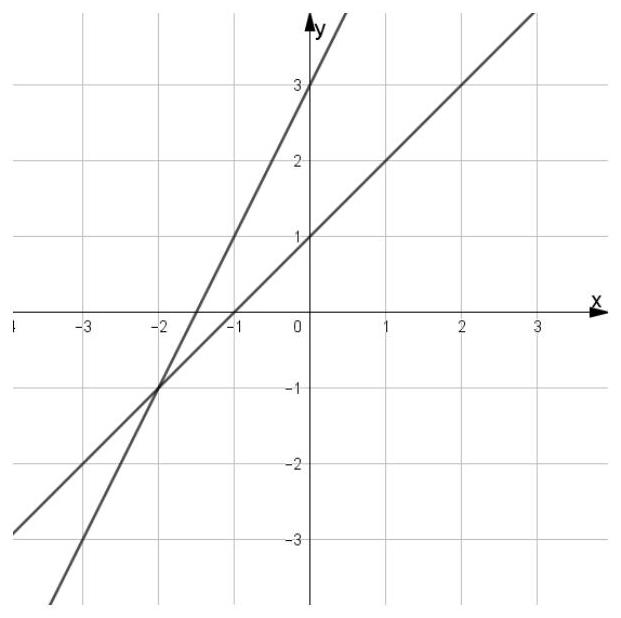
\includegraphics[max width=\textwidth, center]{2024_11_21_fd555512e32c497e8a5dg-04}\\
B.\\
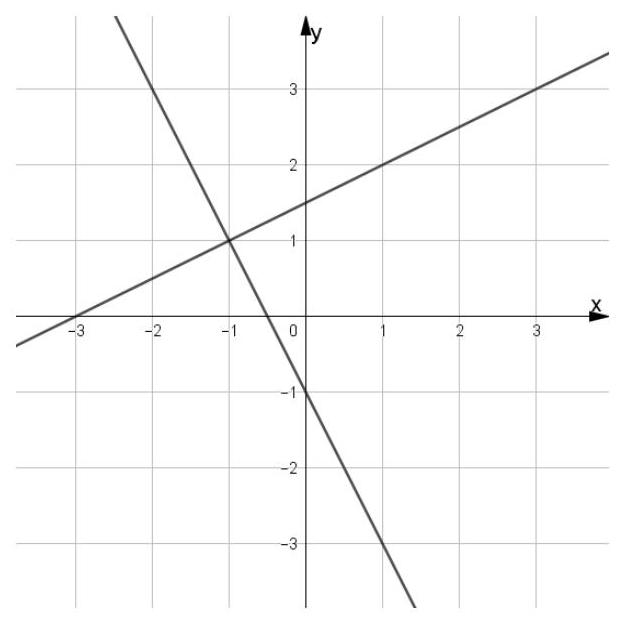
\includegraphics[max width=\textwidth, center]{2024_11_21_fd555512e32c497e8a5dg-04(1)}\\
C.\\
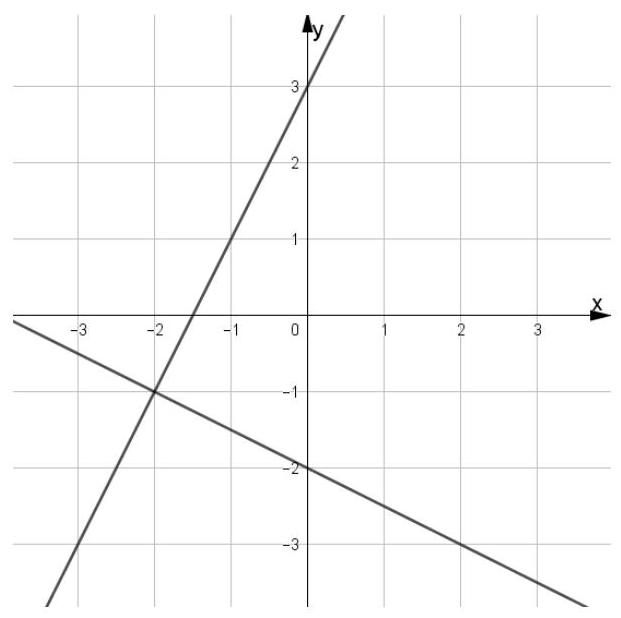
\includegraphics[max width=\textwidth, center]{2024_11_21_fd555512e32c497e8a5dg-04(3)}\\
D.\\
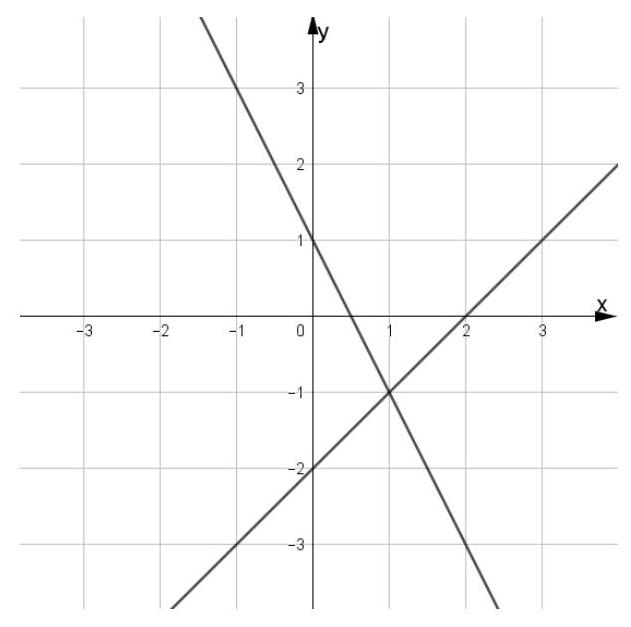
\includegraphics[max width=\textwidth, center]{2024_11_21_fd555512e32c497e8a5dg-04(2)}

Próbny egzamin maturalny z matematyki - POZIOM PODSTAWOWY - MARZEC 2022\\
BRUDNOPIS (nie podlega ocenianiu)\\

\includegraphics[max width=\textwidth, center]{2024_11_21_fd555512e32c497e8a5dg-05}

Próbny egzamin maturalny z matematyki - POZIOM PODSTAWOWY - MARZEC 2022

\section*{Zadanie 10. (0-1)}
Na poniższym rysunku przedstawiono wykres funkcji \(f\) określonej w zbiorze \((-4 ; 4\rangle\).\\
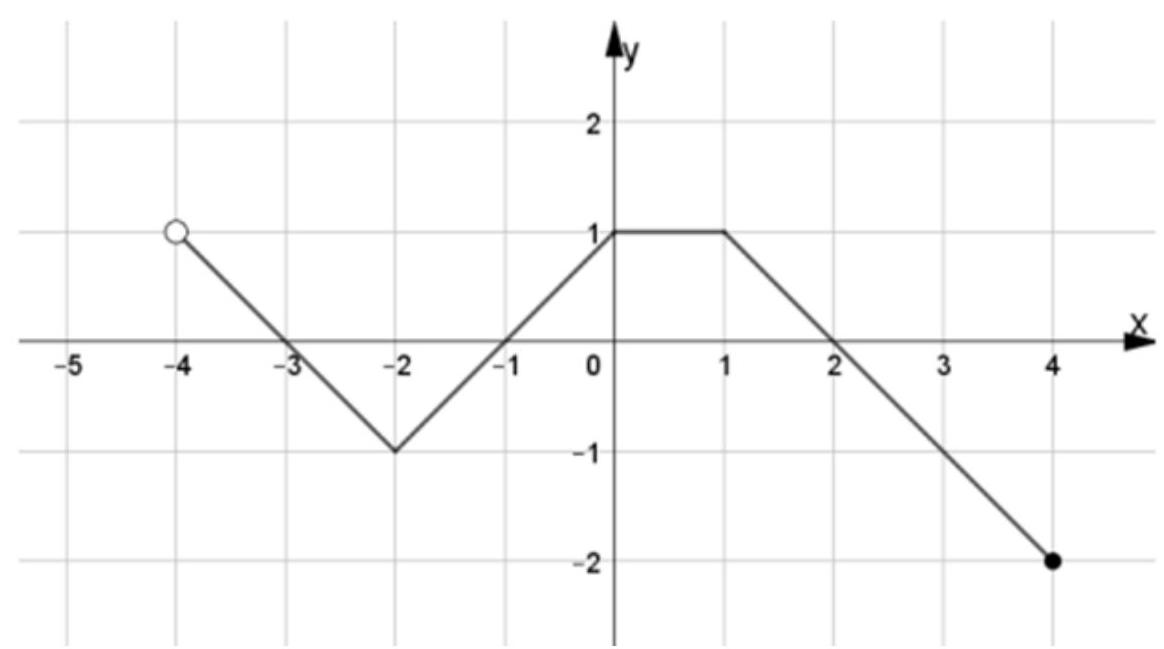
\includegraphics[max width=\textwidth, center]{2024_11_21_fd555512e32c497e8a5dg-06}

Funkcja \(g\) określona jest wzorem \(g(x)=f(x)+1\). Wskaż zdanie prawdziwe.\\
A. Zbiorem wartości funkcji \(g\) jest przedział 〈-1; 2).\\
B. Iloczyn miejsc zerowych funkcji \(g\) jest równy -2 .\\
C. \(f(1) \cdot g(4)=-1\).\\
D. Punkt \(P=(-3 ; 1)\) nie należy do wykresu funkcji \(g\).

\section*{Zadanie 11. (0-1)}
Funkcja \(f\) określona wzorem \(f(x)=-x^{2}-x\) dla każdej liczby rzeczywistej \(x\). Wtedy dla argumentu \(x=-2\) wartość funkcji \(f\) jest równa\\
A. 6\\
B. -6\\
C. 2\\
D. -2

\section*{Zadanie 12. (0-1)}
Punkt \(P=\left(-\frac{1}{2}, 2\right)\) należy do wykresu funkcji \(f(x)=a^{x}\). Wtedy \(a\) jest równe\\
A. \(a=\frac{1}{4}\)\\
B. \(a=4\)\\
C. \(a=2\)\\
D. \(a=\frac{1}{2}\)

\section*{Zadanie 13. (0-1)}
Funkcja kwadratowa \(f\) określona wzorem \(f(x)=-2 x^{2}+4 x-1\) jest rosnąca w przedziale\\
A. \((-\infty ; 1\rangle\)\\
B. \((-\infty ; 4\rangle\)\\
C. \(\langle 4 ;+\infty)\)\\
D. \(\langle 1 ;+\infty)\)

Próbny egzamin maturalny z matematyki - POZIOM PODSTAWOWY - MARZEC 2022\\
BRUDNOPIS (nie podlega ocenianiu)\\

\includegraphics[max width=\textwidth, center]{2024_11_21_fd555512e32c497e8a5dg-07}

Próbny egzamin maturalny z matematyki - POZIOM PODSTAWOWY - MARZEC 2022

\section*{Zadanie 14. (0-1)}
Ciąg arytmetyczny \(\left(a_{n}\right)\) jest określony dla każdej liczby naturalnej \(n \geq 1\). Drugi i szósty wyraz ciągu spełniają warunek \(3 a_{6}-a_{2}=18\). Wtedy ósmy wyraz tego ciągu jest równy\\
A. 3\\
B. 6\\
C. 18\\
D. 9

\section*{Zadanie 15. (0-1)}
Trzywyrazowy ciąg (2, \(-8,3 x\) ) jest geometryczny. Stąd wynika, że\\
A. \(x=-6\)\\
B. \(x=10 \frac{2}{3}\)\\
C. \(x=32\)\\
D. \(x=-\frac{8}{3}\)

\section*{Zadanie 16. (0-1)}
Ciąg \(\left(a_{n}\right)\) jest określony wzorem \(a_{n}=-3(n+2)(n-5)\) dla każdej liczby naturalnej \(n \geq 1\). Liczba dodatnich wyrazów ciągu ( \(a_{n}\) ) jest równa\\
A. 3\\
B. 6\\
C. 5\\
D. 4

\section*{Zadanie 17. (0-1)}
Wartość wyrażenia \(\frac{\sin ^{2} 20^{\circ}+\sin ^{2} 70^{\circ}}{\sin 30^{\circ}}\) jest równa\\
A. 2\\
B. \(\frac{1}{2}\)\\
C. 1\\
D. 4

\section*{Zadanie 18. (0-1)}
Przyprostokątna \(B C\) trójkąta prostokątnego \(A B C\) ma długość 5 oraz \(\sin \alpha=\frac{2}{7}\) (zobacz rysunek).\\
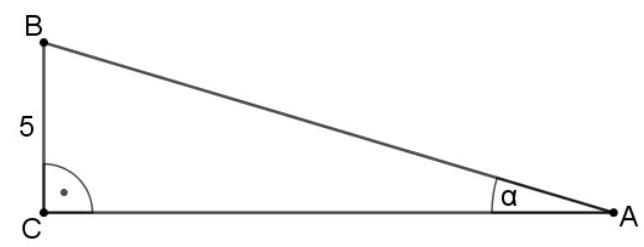
\includegraphics[max width=\textwidth, center]{2024_11_21_fd555512e32c497e8a5dg-08}

Długość przeciwprostokątnej \(A B\) jest równa\\
A. \(\frac{14}{5}\)\\
B. \(\frac{35}{2}\)\\
C. \(\frac{14}{3}\)\\
D. \(\frac{10}{7}\)

\section*{Zadanie 19. (0-1)}
Wykresy funkcji liniowych \(f(x)=3 m x+1\) oraz \(g(x)=4 x+1\) są symetryczne względem osi OY, gdy\\
A. \(m=-\frac{4}{3}\)\\
B. \(m=\frac{4}{3}\)\\
C. \(m=-\frac{1}{12}\)\\
D. \(m=\frac{1}{12}\)

Próbny egzamin maturalny z matematyki - POZIOM PODSTAWOWY - MARZEC 2022\\
BRUDNOPIS (nie podlega ocenianiu)\\

\includegraphics[max width=\textwidth, center]{2024_11_21_fd555512e32c497e8a5dg-09}

\section*{Zadanie 20. (0-1)}
Punkt \(S=\left(-1, \frac{1}{2}\right)\) jest środkiem odcinka \(K L\), w którym punkt \(K=(-7,-2)\). Punkt \(L\) ma współrzędne\\
A. \(\left(-4, \frac{5}{4}\right)\)\\
B. \((5,3)\)\\
C. \(\left(-13,-4 \frac{1}{2}\right)\)\\
D. \((-2,-5)\)

\section*{Zadanie 21. (0-1)}
Punkt \(S\) jest środkiem okręgu przedstawionego na rysunku.\\
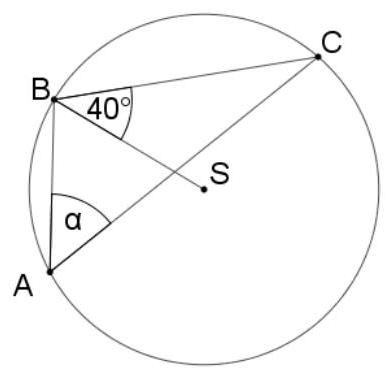
\includegraphics[max width=\textwidth, center]{2024_11_21_fd555512e32c497e8a5dg-10(1)}

Miara kąta \(\alpha\) jest równa\\
A. \(40^{0}\)\\
B. \(50^{0}\)\\
C. \(45^{0}\)\\
D. \(60^{\circ}\)

\section*{Zadanie 22. (0-1)}
W trójkąt równoboczny wpisano dwa koła (tak jak na rysunku). Pole koła o środku \(S_{1}\) oznaczmy \(P_{1}\), a pole koła o środku \(S_{2}\) oznaczmy \(P_{2}\).\\
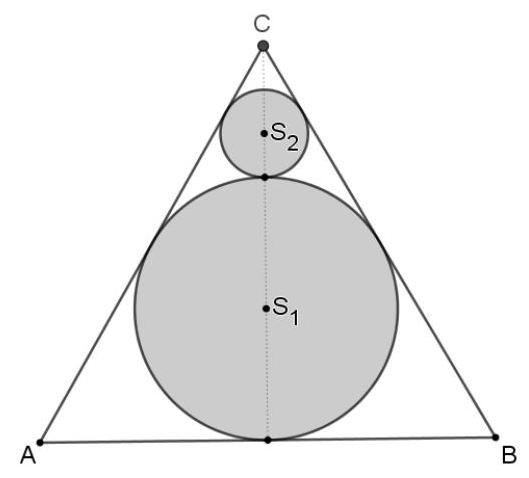
\includegraphics[max width=\textwidth, center]{2024_11_21_fd555512e32c497e8a5dg-10}

Stosunek pól \(\frac{P_{2}}{P_{1}}\) jest równy\\
A. \(\frac{1}{6}\)\\
B. \(\frac{1}{4}\)\\
C. \(\frac{1}{3}\)\\
D. \(\frac{1}{9}\)

Próbny egzamin maturalny z matematyki - POZIOM PODSTAWOWY - MARZEC 2022\\
BRUDNOPIS (nie podlega ocenianiu)

\begin{center}
\begin{tabular}{|c|c|c|c|c|c|c|c|c|c|c|c|c|c|c|c|c|c|c|c|c|c|}
\hline
 &  &  &  &  &  &  &  &  &  &  &  &  &  &  &  &  &  &  &  &  &  \\
\hline
 &  &  &  &  &  &  &  &  &  &  &  &  &  &  &  &  &  &  &  &  &  \\
\hline
 &  &  &  &  &  &  &  &  &  &  &  &  &  &  &  &  &  &  &  &  &  \\
\hline
 &  &  &  &  &  &  &  &  &  &  &  &  &  &  &  &  &  &  &  &  &  \\
\hline
 &  &  &  &  &  &  &  &  &  &  &  &  &  &  &  &  &  &  &  &  &  \\
\hline
 &  &  &  &  &  &  &  &  &  &  &  &  &  &  &  &  &  &  &  &  &  \\
\hline
 &  &  &  &  &  &  &  &  &  &  &  &  &  &  &  &  &  &  &  &  &  \\
\hline
 &  &  &  &  &  &  &  &  &  &  &  &  &  &  &  &  &  &  &  &  &  \\
\hline
 &  &  &  &  &  &  &  &  &  &  &  &  &  &  &  &  &  &  &  &  &  \\
\hline
 &  &  &  &  &  &  &  &  &  &  &  &  &  &  &  &  &  &  &  &  &  \\
\hline
 &  &  &  &  &  &  &  &  &  &  &  &  &  &  &  &  &  &  &  &  &  \\
\hline
 &  &  &  &  &  &  &  &  &  &  &  &  &  &  &  &  &  &  &  &  &  \\
\hline
 &  &  &  &  &  &  &  &  &  &  &  &  &  &  &  &  &  &  &  &  &  \\
\hline
 &  &  &  &  &  &  &  &  &  &  &  &  &  &  &  &  &  &  &  &  &  \\
\hline
 &  &  &  &  &  &  &  &  &  &  &  &  &  &  &  &  &  &  &  &  &  \\
\hline
 &  &  &  &  &  &  &  &  &  &  &  &  &  &  &  &  &  &  &  &  &  \\
\hline
 &  &  &  &  &  &  &  &  &  &  &  &  &  &  &  &  &  &  &  &  &  \\
\hline
 &  &  &  &  &  &  &  &  &  &  &  &  &  &  &  &  &  &  &  &  &  \\
\hline
 &  &  &  &  &  &  &  &  &  &  &  &  &  &  &  &  &  &  &  &  &  \\
\hline
 &  &  &  &  &  &  &  &  &  &  &  &  &  &  &  &  &  &  &  &  &  \\
\hline
 &  &  &  &  &  &  &  &  &  &  &  &  &  &  &  &  &  &  &  &  &  \\
\hline
 &  &  &  &  &  &  &  &  &  &  &  &  &  &  &  &  &  &  &  &  &  \\
\hline
 &  &  &  &  &  &  &  &  &  &  &  &  &  &  &  &  &  &  &  &  &  \\
\hline
 &  &  &  &  &  &  &  &  &  &  &  &  &  &  &  &  &  &  &  &  &  \\
\hline
 &  &  &  &  &  &  &  &  &  &  &  &  &  &  &  &  &  &  &  &  &  \\
\hline
 &  &  &  &  &  &  &  &  &  &  &  &  &  &  &  &  &  &  &  &  &  \\
\hline
 &  &  &  &  &  &  &  &  &  &  &  &  &  &  &  &  &  &  &  &  &  \\
\hline
 &  &  &  &  &  &  &  &  &  &  &  &  &  &  &  &  &  &  &  &  &  \\
\hline
 &  &  &  &  &  &  &  &  &  &  &  &  &  &  &  &  &  &  &  &  &  \\
\hline
 &  &  &  &  &  &  &  &  &  &  &  &  &  &  &  &  &  &  &  &  &  \\
\hline
 &  &  &  &  &  &  &  &  &  &  &  &  &  &  &  &  &  &  &  &  &  \\
\hline
 &  &  &  &  &  &  &  &  &  &  &  &  &  &  &  &  &  &  &  &  &  \\
\hline
 &  &  &  &  &  &  &  &  &  &  &  &  &  &  &  &  &  &  &  &  &  \\
\hline
 &  &  &  &  &  &  &  &  &  &  &  &  &  &  &  &  &  &  &  &  &  \\
\hline
 &  &  &  &  &  &  &  &  &  &  &  &  &  &  &  &  &  &  &  &  &  \\
\hline
 &  &  &  &  &  &  &  &  &  &  &  &  &  &  &  &  &  &  &  &  &  \\
\hline
 &  &  &  &  &  &  &  &  &  &  &  &  &  &  &  &  &  &  &  &  &  \\
\hline
 &  &  &  &  &  &  &  &  &  &  &  &  &  &  &  &  &  &  &  &  &  \\
\hline
 &  &  &  &  &  &  &  &  &  &  &  &  &  &  &  &  &  &  &  &  &  \\
\hline
 &  &  &  &  &  &  &  &  &  &  &  &  &  &  &  &  &  &  &  &  &  \\
\hline
 &  &  &  &  &  &  &  &  &  &  &  &  &  &  &  &  &  &  &  &  &  \\
\hline
 &  &  &  &  &  &  &  &  &  &  &  &  &  &  &  &  &  &  &  &  &  \\
\hline
 &  &  &  &  &  &  &  &  &  &  &  &  &  &  &  &  &  &  &  &  &  \\
\hline
\end{tabular}
\end{center}

Próbny egzamin maturalny z matematyki - POZIOM PODSTAWOWY - MARZEC 2022

\section*{Zadanie 23. (0-1)}
Bok \(A C\) trójkąta \(A B C\) ma długość 4 , pole tego trójkąta jest równe 6 oraz miara kąta \(B A C\) jest równa \(30^{\circ}\) (zobacz rysunek).\\
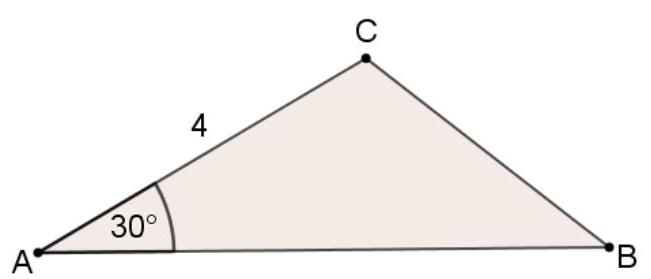
\includegraphics[max width=\textwidth, center]{2024_11_21_fd555512e32c497e8a5dg-12}

Długość boku AB jest równa\\
A. 6\\
B. \(3 \sqrt{3}\)\\
C. 8\\
D. \(6 \sqrt{3}\)

\section*{Zadanie 24. (0-1)}
Prosta k jest styczna w punkcie \(A\) do okręgu o środku \(S\). Punkt B leży na okręgu i miara kąta \(B A S\) jest równa \(40^{\circ}\). Przez punkty \(S\) i \(B\) poprowadzono prostą, która przecina prostą \(k\) w punkcie \(C\). (zobacz rysunek)\\
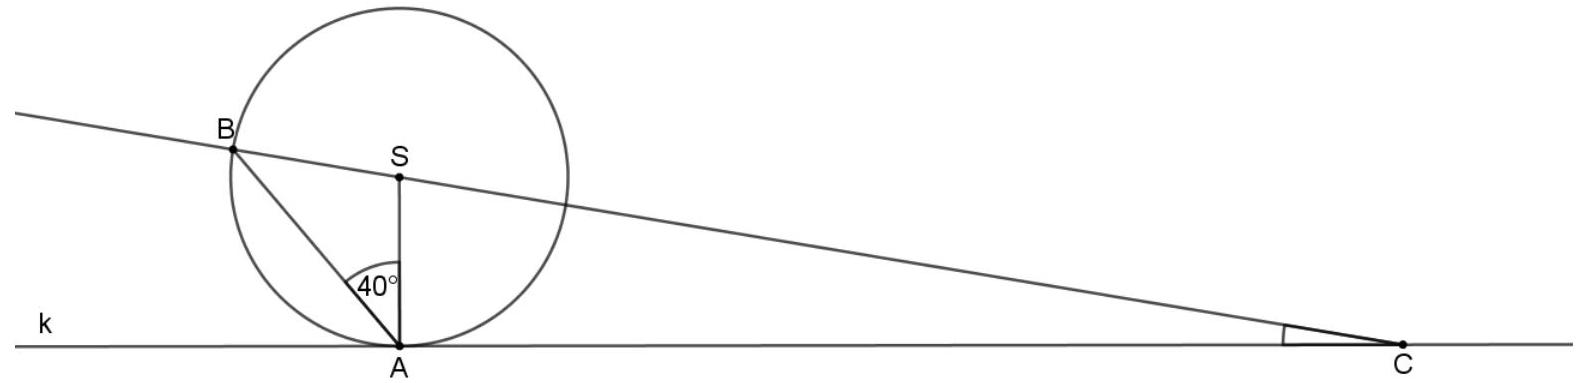
\includegraphics[max width=\textwidth, center]{2024_11_21_fd555512e32c497e8a5dg-12(1)}

Miara kąta \(A C S\) jest równa\\
A. \(15^{0}\)\\
B. \(20^{0}\)\\
C. \(10^{0}\)\\
D. \(40^{\circ}\)

\section*{Zadanie 25. (0-1)}
W graniastosłupie prawidłowym czworokątnym krawędź boczna jest dwa razy dłuższa od krawędzi podstawy. Suma długości wszystkich krawędzi tego graniastosłupa jest równa 64. Przekątna podstawy tego graniastosłupa ma długość\\
A. \(6 \sqrt{3}\)\\
B. \(8 \sqrt{2}\)\\
C. \(4 \sqrt{3}\)\\
D. \(4 \sqrt{2}\)

Próbny egzamin maturalny z matematyki - POZIOM PODSTAWOWY - MARZEC 2022

Zadanie 26. (0-1)\\
Wszystkich liczb naturalnych czterocyfrowych, mniejszych od 5000, w których cyfry mogą się powtarzać oraz każda z cyfr tej liczby należy do zbioru \(\{3,4,5,6\}\), jest\\
A. 192\\
B. 72\\
C. 128\\
D. 18

\section*{Zadanie 27. (0-1)}
Sześciowyrazowy ciąg liczbowy ( \(0,3,5, x, 10,11\) ) jest rosnący. Średnia arytmetyczna wyrazów tego ciągu jest równa medianie. Wynika stąd, że mediana wyrazów tego ciągu jest równa\\
A. 6\\
B. 7\\
C. 8\\
D. 9

\section*{Zadanie 28. (0-1)}
Ze zbioru liczb naturalnych dwucyfrowych mniejszych od 25 losujemy jedną liczbę. Prawdopodobieństwo wylosowania liczby podzielnej przez 6 jest równe\\
A. \(\frac{4}{25}\)\\
B. \(\frac{1}{8}\)\\
C. \(\frac{3}{14}\)\\
D. \(\frac{1}{5}\)

BRUDNOPIS (nie podlega ocenie)

\begin{center}
\begin{tabular}{|c|c|c|c|c|c|c|c|c|c|c|c|c|c|c|c|c|c|c|c|c|c|c|c|c|c|c|c|c|c|}
\hline
 &  &  &  &  &  &  &  &  &  &  &  &  &  &  &  &  &  &  &  &  &  &  &  &  &  &  &  &  &  \\
\hline
 &  &  &  &  &  &  &  &  &  &  &  &  &  &  &  &  &  &  &  &  &  &  &  &  &  &  &  &  &  \\
\hline
 &  &  &  &  &  &  &  &  &  &  &  &  &  &  &  &  &  &  &  &  &  &  &  &  &  &  &  &  &  \\
\hline
 &  &  &  &  &  &  &  &  &  &  &  &  &  &  &  &  &  &  &  &  &  &  &  &  &  &  &  &  &  \\
\hline
 &  &  &  &  &  &  &  &  &  &  &  &  &  &  &  &  &  &  &  &  &  &  &  &  &  &  &  &  &  \\
\hline
 &  &  &  &  &  &  &  &  &  &  &  &  &  &  &  &  &  &  &  &  &  &  &  &  &  &  &  &  &  \\
\hline
 &  &  &  &  &  &  &  &  &  &  &  &  &  &  &  &  &  &  &  &  &  &  &  &  &  &  &  &  &  \\
\hline
 &  &  &  &  &  &  &  &  &  &  &  &  &  &  &  &  &  &  &  &  &  &  &  &  &  &  &  &  &  \\
\hline
 &  &  &  &  &  &  &  &  &  &  &  &  &  &  &  &  &  &  &  &  &  &  &  &  &  &  &  &  &  \\
\hline
 &  &  &  &  &  &  &  &  &  &  &  &  &  &  &  &  &  &  &  &  &  &  &  &  &  &  &  &  &  \\
\hline
 &  &  &  &  &  &  &  &  &  &  &  &  &  &  &  &  &  &  &  &  &  &  &  &  &  &  &  &  &  \\
\hline
 &  &  &  &  &  &  &  &  &  &  &  &  &  &  &  &  &  &  &  &  &  &  &  &  &  &  &  &  &  \\
\hline
 &  &  &  &  &  &  &  &  &  &  &  &  &  &  &  &  &  &  &  &  &  &  &  &  &  &  &  &  &  \\
\hline
 &  &  &  &  &  &  &  &  &  &  &  &  &  &  &  &  &  &  &  &  &  &  &  &  &  &  &  &  &  \\
\hline
 &  &  &  &  &  &  &  &  &  &  &  &  &  &  &  &  &  &  &  &  &  &  &  &  &  &  &  &  &  \\
\hline
 &  &  &  &  &  &  &  &  &  &  &  &  &  &  &  &  &  &  &  &  &  &  &  &  &  &  &  &  &  \\
\hline
 &  &  &  &  &  &  &  &  &  &  &  &  &  &  &  &  &  &  &  &  &  &  &  &  &  &  &  &  &  \\
\hline
 &  &  &  &  &  &  &  &  &  &  &  &  &  &  &  &  &  &  &  &  &  &  &  &  &  &  &  &  &  \\
\hline
 &  &  &  &  &  &  &  &  &  &  &  &  &  &  &  &  &  &  &  &  &  &  &  &  &  &  &  &  &  \\
\hline
 &  &  &  &  &  &  &  &  &  &  &  &  &  &  &  &  &  &  &  &  &  &  &  &  &  &  &  &  &  \\
\hline
 & - &  &  &  &  &  &  &  &  &  &  &  &  &  &  &  &  &  &  &  &  &  &  &  &  &  &  &  &  \\
\hline
 & - &  &  &  &  &  &  &  &  &  &  &  &  &  &  &  &  &  &  &  &  &  &  &  &  &  &  &  &  \\
\hline
 & - &  &  &  &  &  &  &  &  &  &  &  &  &  &  &  &  &  &  &  &  &  &  &  &  &  &  &  &  \\
\hline
 &  &  &  &  &  &  &  &  &  &  &  &  &  &  &  &  &  &  &  &  &  &  &  &  &  &  &  &  &  \\
\hline
\end{tabular}
\end{center}

\section*{ZADANIA OTWARTE}
Rozwiqzania zadań o numerach od 26. do 34. należy zapisać w wyznaczonych miejscach pod treściq zadania. Zadanie 29. (0-2)

Rozwiąż nierówność \(2-(x-3)(x+2) \geq-4\)\\

\includegraphics[max width=\textwidth, center]{2024_11_21_fd555512e32c497e8a5dg-14}

Odpowiedź\\
Zadanie 30. (0-2)\\
Rozwiąż równanie \(-5\left(2 x^{2}-18\right)\left(x^{2}+32\right)=0\).

\begin{center}
\begin{tabular}{|c|c|c|c|c|c|c|c|c|c|c|c|c|c|c|c|c|c|c|c|c|c|c|c|c|c|c|c|c|c|}
\hline
 &  &  &  &  &  &  &  &  &  &  &  &  &  &  &  &  &  &  &  &  &  &  &  &  &  &  &  &  &  \\
\hline
 &  &  &  &  &  &  &  &  &  &  &  &  &  &  &  &  &  &  &  &  &  &  &  &  &  &  &  &  &  \\
\hline
 &  &  &  &  &  &  &  &  &  &  &  &  &  &  &  &  &  &  &  &  &  &  &  &  &  &  &  &  &  \\
\hline
 &  &  &  &  &  &  &  &  &  &  &  &  &  &  &  &  &  &  &  &  &  &  &  &  &  &  &  &  &  \\
\hline
 &  &  &  &  &  &  &  &  &  &  &  &  &  &  &  &  &  &  &  &  &  &  &  &  &  &  &  &  &  \\
\hline
 &  &  &  &  &  &  &  &  &  &  &  &  &  &  &  &  &  &  &  &  &  &  &  &  &  &  &  &  &  \\
\hline
 &  &  &  &  &  &  &  &  &  &  &  &  &  &  &  &  &  &  &  &  &  &  &  &  &  &  &  &  &  \\
\hline
 &  &  &  &  &  &  &  &  &  &  &  &  &  &  &  &  &  &  &  &  &  &  &  &  &  &  &  &  &  \\
\hline
 &  &  &  &  &  &  &  &  &  &  &  &  &  &  &  &  &  &  &  &  &  &  &  &  &  &  &  &  &  \\
\hline
 &  &  &  &  &  &  &  &  &  &  &  &  &  &  &  &  &  &  &  &  &  &  &  &  &  &  &  &  &  \\
\hline
 &  &  &  &  &  &  &  &  &  &  &  &  &  &  &  &  &  &  &  &  &  &  &  &  &  &  &  &  &  \\
\hline
 &  &  &  &  &  &  &  &  &  &  &  &  &  &  &  &  &  &  &  &  &  &  &  &  &  &  &  &  &  \\
\hline
 &  &  &  &  &  &  &  &  &  &  &  &  &  &  &  &  &  &  &  &  &  &  &  &  &  &  &  &  &  \\
\hline
 &  &  &  &  &  &  &  &  &  &  &  &  &  &  &  &  &  &  &  &  &  &  &  &  &  &  &  &  &  \\
\hline
 &  &  &  &  &  &  &  &  &  &  &  &  &  &  &  &  &  &  &  &  &  &  &  &  &  &  &  &  &  \\
\hline
 &  &  &  &  &  &  &  &  &  &  &  &  &  &  &  &  &  &  &  &  &  &  &  &  &  &  &  &  &  \\
\hline
 &  &  &  &  &  &  &  &  &  &  &  &  &  &  &  &  &  &  &  &  &  &  &  &  &  &  &  &  &  \\
\hline
\end{tabular}
\end{center}

Odpowiedź \(\qquad\)

\section*{Zadanie 31. (0-2)}
Uzasadnij, że dla dowolnych liczb rzeczywistych \(a\) i \(b\) spełniona jest nierówność

\[
a^{2}+2 b^{2}>2 a b-1
\]

\begin{center}

\includegraphics[max width=\textwidth]{2024_11_21_fd555512e32c497e8a5dg-15}
\end{center}

Próbny egzamin maturalny z matematyki - POZIOM PODSTAWOWY - MARZEC 2022

Zadanie 32. (0-2)\\
Przekątna \(A C\) o długości 6 jest wysokością trapezu \(A B C D\). Miara kąta \(A B C\) jest równa \(30^{\circ}\). Bok \(B C\) oraz podstawa \(C D\) mają równe długości (zobacz rysunek).\\
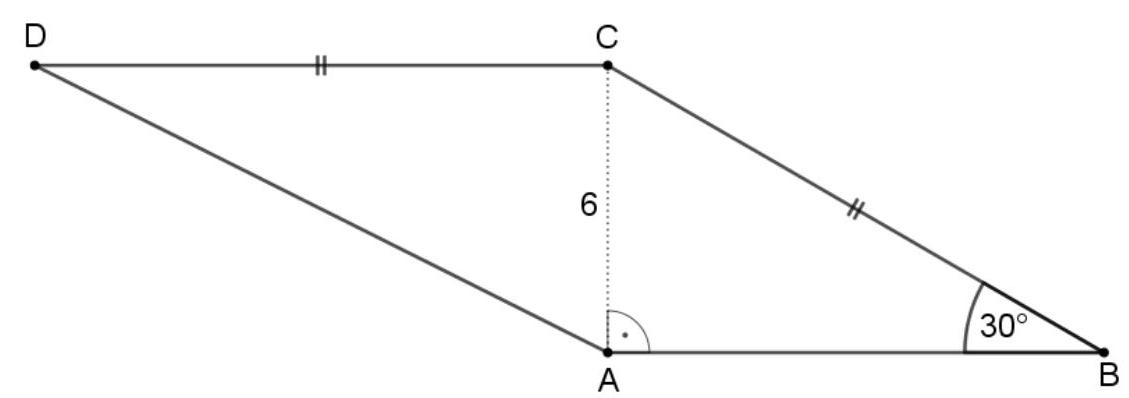
\includegraphics[max width=\textwidth, center]{2024_11_21_fd555512e32c497e8a5dg-16}

Oblicz długość boku \(A D\).\\

\includegraphics[max width=\textwidth, center]{2024_11_21_fd555512e32c497e8a5dg-16(1)}

Odpowiedź

Próbny egzamin maturalny z matematyki - POZIOM PODSTAWOWY - MARZEC 2022

\section*{Zadanie 33. (0-2)}
Liczby \(\quad x, \quad x^{2}+1,8 x-2 \quad\) w podanej kolejności są pierwszym, drugim i piątym wyrazem ciągu arytmetycznego. Oblicz \(x\).

\begin{center}
\begin{tabular}{|c|c|c|c|c|c|c|c|c|c|c|c|c|c|c|c|c|c|c|c|c|c|c|c|}
\hline
 &  &  &  &  &  &  &  &  &  &  &  &  &  &  &  &  &  &  &  &  &  &  &  \\
\hline
 &  &  &  &  &  &  &  &  &  &  &  &  &  &  &  &  &  &  &  &  &  &  &  \\
\hline
 &  &  &  &  &  &  &  &  &  &  &  &  &  &  &  &  &  &  &  &  &  &  &  \\
\hline
 &  &  &  &  &  &  &  &  &  &  &  &  &  &  &  &  &  &  &  &  &  &  &  \\
\hline
 &  &  &  &  &  &  &  &  &  &  &  &  &  &  &  &  &  &  &  &  &  &  &  \\
\hline
 &  &  &  &  &  &  &  &  &  &  &  &  &  &  &  &  &  &  &  &  &  &  &  \\
\hline
 &  &  &  &  &  &  &  &  &  &  &  &  &  &  &  &  &  &  &  &  &  &  &  \\
\hline
 &  &  &  &  &  &  &  &  &  &  &  &  &  &  &  &  &  &  &  &  &  &  &  \\
\hline
 &  &  &  &  &  &  &  &  &  &  &  &  &  &  &  &  &  &  &  &  &  &  &  \\
\hline
 &  &  &  &  &  &  &  &  &  &  &  &  &  &  &  &  &  &  &  &  &  &  &  \\
\hline
 &  &  &  &  &  &  &  &  &  &  &  &  &  &  &  &  &  &  &  &  &  &  &  \\
\hline
 &  &  &  &  &  &  &  &  &  &  &  &  &  &  &  &  &  &  &  &  &  &  &  \\
\hline
 &  &  &  &  &  &  &  &  &  &  &  &  &  &  &  &  &  &  &  &  &  &  &  \\
\hline
 &  &  &  &  &  &  &  &  &  &  &  &  &  &  &  &  &  &  &  &  &  &  &  \\
\hline
 &  &  &  &  &  &  &  &  &  &  &  &  &  &  &  &  &  &  &  &  &  &  &  \\
\hline
 &  &  &  &  &  &  &  &  &  &  &  &  &  &  &  &  &  &  &  &  &  &  &  \\
\hline
 &  &  &  &  &  &  &  &  &  &  &  &  &  &  &  &  &  &  &  &  &  &  &  \\
\hline
 &  &  &  &  &  &  &  &  &  &  &  &  &  &  &  &  &  &  &  &  &  &  &  \\
\hline
 &  &  &  &  &  &  &  &  &  &  &  &  &  &  &  &  &  &  &  &  &  &  &  \\
\hline
 &  &  &  &  &  &  &  &  &  &  &  &  &  &  &  &  &  &  &  &  &  &  &  \\
\hline
 &  &  &  &  &  &  &  &  &  &  &  &  &  &  &  &  &  &  &  &  &  &  &  \\
\hline
 &  &  &  &  &  &  &  &  &  &  &  &  &  &  &  &  &  &  &  &  &  &  &  \\
\hline
 &  &  &  &  &  &  &  &  &  &  &  &  &  &  &  &  &  &  &  &  &  &  &  \\
\hline
 &  &  &  &  &  &  &  &  &  &  &  &  &  &  &  &  &  &  &  &  &  &  &  \\
\hline
 &  &  &  &  &  &  &  &  &  &  &  &  &  &  &  &  &  &  &  &  &  &  &  \\
\hline
 &  &  &  &  &  &  &  &  &  &  &  &  &  &  &  &  &  &  &  &  &  &  &  \\
\hline
 &  &  &  &  &  &  &  &  &  &  &  &  &  &  &  &  &  &  &  &  &  &  &  \\
\hline
 &  &  &  &  &  &  &  &  &  &  &  &  &  &  &  &  &  &  &  &  &  &  &  \\
\hline
 &  &  &  &  &  &  &  &  &  &  &  &  &  &  &  &  &  &  &  &  &  &  &  \\
\hline
 &  &  &  &  &  &  &  &  &  &  &  &  &  &  &  &  &  &  &  &  &  &  &  \\
\hline
 &  &  &  &  &  &  &  &  &  &  &  &  &  &  &  &  &  &  &  &  &  &  &  \\
\hline
 &  &  &  &  &  &  &  &  &  &  &  &  &  &  &  &  &  &  &  &  &  &  &  \\
\hline
 &  &  &  &  &  &  &  &  &  &  &  &  &  &  &  &  &  &  &  &  &  &  &  \\
\hline
 &  &  &  &  &  &  &  &  &  &  &  &  &  &  &  &  &  &  &  &  &  &  &  \\
\hline
 &  &  &  &  &  &  &  &  &  &  &  &  &  &  &  &  &  &  &  &  &  &  &  \\
\hline
 &  &  &  &  &  &  &  &  &  &  &  &  &  &  &  &  &  &  &  &  &  &  &  \\
\hline
 &  &  &  &  &  &  &  &  &  &  &  &  &  &  &  &  &  &  &  &  &  &  &  \\
\hline
 &  &  &  &  &  &  &  &  &  &  &  &  &  &  &  &  &  &  &  &  &  &  &  \\
\hline
\end{tabular}
\end{center}

Próbny egzamin maturalny z matematyki - POZIOM PODSTAWOWY - MARZEC 2022

\section*{Zadanie 34. (0-2)}
Punkt \(W=(-2.4)\) jest wierzchołkiem paraboli będącej wykresem funkcji kwadratowej \(f(x)=-2 x^{2}+b x+c\). Wyznacz wartości współczynników \(b\) oraz \(c\).\\

\includegraphics[max width=\textwidth, center]{2024_11_21_fd555512e32c497e8a5dg-18}

Odpowiedź

Próbny egzamin maturalny z matematyki - POZIOM PODSTAWOWY - MARZEC 2022

Zadanie 35. (0-5)\\
Punkty \(A=(-3,-2)\) oraz \(B=(1,4)\) są wierzchołkami trójkąta równoramiennego \(A B P\), w którym \(|A P|=|B P|\). Punkt \(P\) leży na prostej \(y=\frac{1}{2} x-9\). Wyznacz współrzędne punktu \(P\) oraz długość odcinka \(A P\).\\

\includegraphics[max width=\textwidth, center]{2024_11_21_fd555512e32c497e8a5dg-19}

Odpowiedź \(\qquad\)

KARTA ODPOWIEDZI

WYPEŁNIA ZDAJĄCY\\
PESEL\\
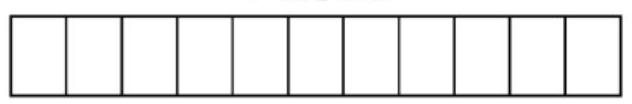
\includegraphics[max width=\textwidth, center]{2024_11_21_fd555512e32c497e8a5dg-20}

\begin{center}
\begin{tabular}{|c|c|c|c|c|}
\hline
\(\underset{\text { zadania }}{\substack{\mathrm{N} \\ \text { and }}}\) & \multicolumn{4}{|c|}{ODPOWIEDZI} \\
\hline
1 & A & B & (c) & D \\
\hline
2 & A & B & (c) & D \\
\hline
3 & A & B & (c) & D \\
\hline
4 & A & B & (c) & D \\
\hline
5 & A & B & (c) & D \\
\hline
6 & A & B & (c) & D \\
\hline
7 & A & B & (c) & D \\
\hline
8 & A & B & (c) & D \\
\hline
9 & A & B & (c) & D \\
\hline
10 & A & B & (c) & D \\
\hline
11 & A & B & (c) & D \\
\hline
12 & A & B & (c) & D \\
\hline
13 & A & B & (c) & D \\
\hline
14 & A & B & (c) & D \\
\hline
\end{tabular}
\end{center}

\begin{center}
\begin{tabular}{|c|c|c|c|c|}
\hline
\(\stackrel{\text { Nr }}{\text { zadania }}\) & \multicolumn{4}{|c|}{ODPOWIEDZI} \\
\hline
15 & A & B & (c) & D \\
\hline
16 & A & B & (c) & D \\
\hline
17 & A & B & (c) & D \\
\hline
18 & A & B & (c) & D \\
\hline
19 & A & B & (c) & D \\
\hline
20 & A & B & (c) & D \\
\hline
21 & A & B & (c) & D \\
\hline
22 & A & (B) & (c) & D \\
\hline
23 & A & (B) & (c) & D \\
\hline
24 & A & B & (c) & D \\
\hline
25 & A & B & (c) & D \\
\hline
26 & A & B & (c) & D \\
\hline
27 & A & B & (c) & D \\
\hline
28 & A & (B) & (c) & D \\
\hline
\end{tabular}
\end{center}


\end{document}